
\documentclass[11pt]{article}
%\usepackage[top=20mm,left=20mm,right=20mm,bottom=15mm,a4paper]{geometry} % see geometry.pdf on how to lay out the page. There's lots.
\usepackage[top=20mm,left=20mm,right=20mm,bottom=15mm,headsep=15pt,footskip=15pt,a4paper]{geometry} % see geometry.pdf on how to lay out the page. There's lots.
%\geometry{a4paper} % or letter or a5paper or ... etc
% \geometry{landscape} % rotated page geometry
\usepackage[round]{natbib}
\setlength{\bibsep}{0.0pt}
\usepackage{color}
\usepackage{times}
%\usepackage[T1]{fontenc}
%\usepackage{mathptmx}
\usepackage{tikz-dependency}
\usepackage{enumitem}
%\usepackage{times}

\usepackage[procnames]{listings}
\usepackage{color}
 
 

% See the ``Article customise'' template for come common customisations
\newcommand{\refeq}[1]{Equation~\ref{eq:#1}}
\newcommand{\reffig}[1]{Figure~\ref{fig:#1}}
\newcommand{\reftab}[1]{Table~\ref{tab:#1}}
\newcommand{\refsec}[1]{\textsection\ref{sec:#1}}
\newcommand{\newsec}[2]{\section{#1}\label{sec:#2}\noindent}
\newcommand{\newsubsec}[2]{\subsection{#1}\label{sec:#2}\noindent}
\newcommand{\argmax}{\operatornamewithlimits{argmax}} 
\newcommand{\argmin}{\operatornamewithlimits{argmin}} 

\makeatletter         
\def\@maketitle{   % custom maketitle 
\begin{center}%
{\bfseries \@title}%
{\bfseries \@author}%
\end{center}%
\smallskip \hrule \bigskip }

% custom section 
\renewcommand{\section}{\@startsection
{section}%                   % the name
{1}%                         % the level
{0mm}%                       % the indent
{-0.8\baselineskip}%            % the before skip
{0.3\baselineskip}%          % the after skip
{\bfseries\large}}% the style

% custom subsection 
\renewcommand{\subsection}{\@startsection
{subsection}%                   % the name
{2}%                         % the level
{0mm}%                       % the indent
{-0.8\baselineskip}%            % the before skip
{0.3\baselineskip}%          % the after skip
{\bfseries\large}}% the style

\renewcommand{\paragraph}{%
  \@startsection{paragraph}{4}%
  {\z@}{1.5ex \@plus 1ex \@minus .2ex}{-1em}%
  {\normalfont\normalsize\bfseries}%
}\makeatother

%\title{{\LARGE Universal Parser (UP)}\\[-8mm]
%\includegraphics[height=8mm]{RUPA}~~~~~~~~~~~~~~~~~~~~~~~~~~~~~~~~~~~~~~~~~~~~~~~~~~~~~~~~~~~~~~~~~~~~~~~~~~~\includegraphics[height=8mm]{RUPA}}
\title{{\LARGE Natural Language Processing}\\[1.5mm]{\large Assignment 8: Treebank Grammars}}
\author{}
\date{} % delete this line to display the current date

%%% BEGIN DOCUMENT
\begin{document}

\definecolor{keywords}{RGB}{255,0,90}
\definecolor{comments}{RGB}{0,0,113}
\definecolor{red}{RGB}{160,0,0}
\definecolor{green}{RGB}{0,150,0}
 
\lstset{language=Python, 
        basicstyle=\ttfamily\small, 
        keywordstyle=\color{keywords},
        commentstyle=\color{comments},
        stringstyle=\color{red},
        showstringspaces=false,
        identifierstyle=\color{green},
        procnamekeys={def,class}}

\maketitle
%\tableofcontents
%\vspace{3mm}
\vspace{-2mm} \newsec{Introduction}{intro}%
The main task in this assignment is to extract a (probabilistic)
context-free grammar from a treebank of English. In the process, we
will also get acquainted with a number of concepts relating to
grammars and treebanks. To facilitate the work, we will make use of
NLTK (Natural Language Toolkit), a Python platform for NLP that
contains a number of useful modules for working with treebanks and
grammars, as well as a subsection of the Penn Treebank for
English. NLTK is installed on our linux system, and all additional
files needed can be found in {\tt /local/kurs/nlp/syntax/}.

\newsec{Explore the treebank (4 P)}{data}%
The Penn Treebank of English is one of the most widely used
syntactically annotated corpora in the field of NLP. Unfortunately, it
is not freely available, but the NLTK distribution contains a sample
of about 4,000 trees, which represents about 10\% of the Wall Street
Journal section of the treebank. We will start by exploring this data
set using the interactive Python interpreter.

\begin{center}
\fbox{
\lstinputlisting{code/explore_tree.py}
}
\end{center}
The above listing shows how to import the treebank from the {\tt
  nltk.corpus} module,\footnote{An overview of the corpora available
  in NLTK can be found at {\tt http://www.nltk.org/nltk\_data/}.}  get
a list of all syntactic trees using the method {\tt
  treebank.parsed\_sents()} and then printing the first tree in that
list. The {\tt draw()} method associated with a tree object can be
used to open a graphical viewer that displays the tree as shown below.

\begin{center}
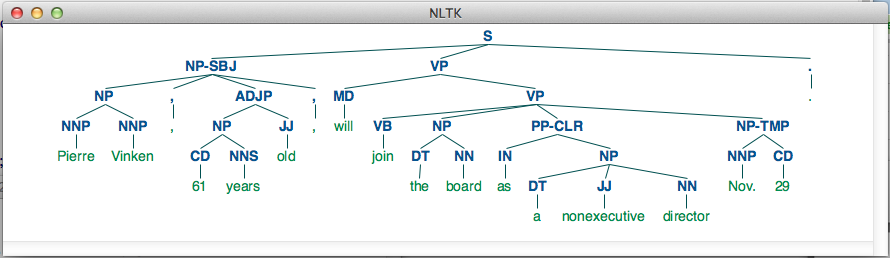
\includegraphics[scale=0.45]{pics/nltk_tree}
\end{center}
Inspect the first tree (and as many additional trees as you like) and
make sure that you understand the phrase structure
representation. Then answer the following questions about the first
tree: \newpage
\begin{enumerate}[noitemsep,topsep=0.2cm]
\item (1 P) What is the symbol on the root node? [Try {\tt t.label()}.]
\item (1 P) How many leaf nodes are there? List them. [Try {\tt t.leaves()}.]
\item (1 P) How many nonterminal symbols are there? List them.
\item (1 P) How many different context-free rules are used in the tree? List them. [Try {\tt t.productions()}.]\label{grammar}
\end{enumerate}

\newsec{Extract a grammar (16 P)}{cfg}%
If we have a phrase structure treebank, we can extract a context-free
grammar by simply reading off all the rules that are needed to
generate all the trees in the treebank.  In fact, in answering
question~\ref{grammar} above, you already extracted a mini-grammar
that generates the first tree in the treebank (and many other trees as
well).  We will now extend this method to a larger portion of the
treebank and add probabilities to grammar rules, but to keep things
manageable we will only use the first 1000 sentences of the treebank.
Moreover, we will simplify the representation by stripping off
anything that occurs after the basic syntactic category of a
node. Thus, symbols like {\tt NP}, {\tt NP-SBJ} and {\tt NP-SBJ-1}
will all be mapped to {\tt NP}. We will also ignore so-called empty
nodes, which are assigned the category {\tt -NONE-} in the Penn
Treebank.  Finally, we will map the fine-grained part-of-speech tags
to the 17 universal tags that we used in the part-of-speech tagging
assignment.  NLTK provides tools for extracting grammars from
treebanks, and to facilitate your work we have built a little package
called {\tt treebank\_grammar.py}

\begin{center}
\fbox{
\lstinputlisting{code/extract_grammar.py}
}
\end{center}
After importing {\tt treebank\_grammar} (and calling it {\tt tg}) for
convenience, we extract a probabilistic context-free grammar using the
method {\tt tg.extract\_simple\_pcfg(1000)}, whose single argument
specifies the number of treebank sentences to use. The method {\tt
  tg.print\_grammar(g, "PP")} can then be used to print all the rules
with the same left-hand side ({\tt PP} in the example). If you want to
print the entire grammar, just omit the second argument: {\tt
  tg.print\_grammar(g)}. Use these methods to explore the grammar and
answer the following questions. Note however that you will either have
to adapt the methods or print their output to files and explore them
with the commandline (e.g. using {\tt grep} as in Assignment 3).
\begin{enumerate}[topsep=0.2cm,itemsep=0cm]
\item (3 P) How many distinct rules are there for the categories {\tt
    S}, {\tt NP} and {\tt VP}, respectively?
\item (3 P) Find the three most probable rules for {\tt S}, {\tt NP}
  and {\tt VP}, and construct real phrases that instantiate them.  For
  example, the rule {\tt VP -> VERB SBAR} is instantiated by the
  phrase ``says that she must go''.
\item Consider the sentence: ``The rates rise .''
  \begin{enumerate}[noitemsep,topsep=0cm]
  \item (3 P) Based on the tags which the grammar can assign to each
    word of the sentence, how many tag sequences are possible? Please
    explain your answer.\\
    \textbf{[VG]} Check for each possible tag sequence if the grammar
    actually can construct a parse tree for it. Explain your reasoning.
%  \item (3 P) How many distinct tag sequences does the grammar assign
%    to the sentence? Explain.
\item (3 P) Construct at least one complete parse tree (with the root
  symbol {\tt S}) for the sentence.
\item (2 P) Do you consider the sentence syntactically ambiguous?
\item (2 P) \textbf{Guess} how many distinct parse trees the sentence
  has according to the grammar?
\end{enumerate}
\end{enumerate}

\newsec{Submit the assignment}{sub}%
Upload the following to {\it Studentportalen}
\textbf{before 20:00h December 2nd}. In order to pass you must provide
answers to all exercises and achieve at least 15/20 points.
\begin{itemize}[noitemsep,topsep=0.2cm]
\item Well motivated answers to all questions in
  Section~\ref{sec:data}--\ref{sec:cfg} (\texttt{.pdf} format, written
  in \LaTeX.
\item \textbf{[VG]}: In order to get the grade VG, reach at least 18
  points in the exercises above and answer the VG condition for question                     
  3.a.
\end{itemize}

\end{document}
